\documentclass[tikz, border=6pt]{standalone}
\usepackage{amsmath,amssymb,bm}
\usepackage{newtxtext,newtxmath}   % Times-like text and math
\usepackage{tikz}
\usepackage{graphicx}
\usetikzlibrary{shapes.geometric, arrows.meta, positioning, calc, fit, backgrounds, shapes.symbols}
\definecolor{cExpert}{HTML}{8C8C8C}
\definecolor{cPolicy}{HTML}{E07B1A}
\definecolor{cCal}{HTML}{3B7DD1}
\definecolor{cBlend}{HTML}{4A8FD6}
\definecolor{cTrain}{HTML}{9DC08B}
\definecolor{cCollect}{HTML}{F5C08A}
\definecolor{cData}{HTML}{E9E9E9}
\definecolor{cBase}{HTML}{F1E4B8}
\definecolor{cOpen}{HTML}{B08BC9}
\definecolor{cOpenLine}{HTML}{7A4F96}
\definecolor{cLab1}{HTML}{F2A541}
\definecolor{cLab2}{HTML}{E0821F}
\definecolor{cLab3}{HTML}{C95D08}
\begin{document}
\begin{tikzpicture}[
  >=Stealth, font=\rmfamily,
  block/.style={rectangle, rounded corners=8pt, minimum height=1.55cm, align=center, font=\rmfamily\bfseries\small, inner sep=7pt, text width=3.5cm},
  data/.style={cylinder, shape border rotate=90, aspect=0.25, draw=black!65, line width=0.8pt, fill=cData, minimum width=1.5cm, minimum height=1.1cm, align=center, font=\rmfamily\small, inner sep=2pt},
  flow/.style={-{Latex[scale=1.2]}, line width=1.6pt, draw=black!60},
  loop/.style={-{Latex[scale=1.2]}, line width=1.4pt, draw=black!60, rounded corners=8pt},
  lab/.style={font=\rmfamily\scriptsize, align=center},
  paneltitle/.style={font=\rmfamily\bfseries\scriptsize, align=center, text width=3.9cm},
  formula/.style={font=\scriptsize, align=center, text width=3.9cm},
  region/.style={rounded corners=14pt, inner sep=8pt},
  chip/.style={rectangle, rounded corners=3pt, draw=cTrain!60!black, fill=cTrain!45, font=\rmfamily\bfseries\scriptsize, inner sep=2.5pt, minimum height=0.42cm}
]
% ================= Row 1: the DAgger loop =================
\node[data, fill=cBase] (D0) at (0,0) {Base\\demos $\mathcal{D}_0$};
\node[block, fill=cTrain!60, right=0.9cm of D0] (train) {Train / fine-tune\\policy $\pi_\theta$};
\node[block, fill=cCollect!70, right=1.1cm of train, text width=4.9cm] (collect) {Roll out $\pi_\theta$ in simulation;\\expert takes over on\\predicted failure};
\node[data, fill=cCollect!45, right=0.9cm of collect] (Dk) {Interventions\\$\mathcal{D}_k$};
\draw[flow] (D0) -- (train);
\draw[flow] (train) -- (collect);
\draw[flow] (collect) -- (Dk);

% ================= Row 2: real calibration panels (Fig. 4 data) inside the box =================
\coordinate (rowy) at (0,-4.35);
\node[inner sep=0, anchor=north west] (panels) at ($(rowy)+(2.9,1.55)$) {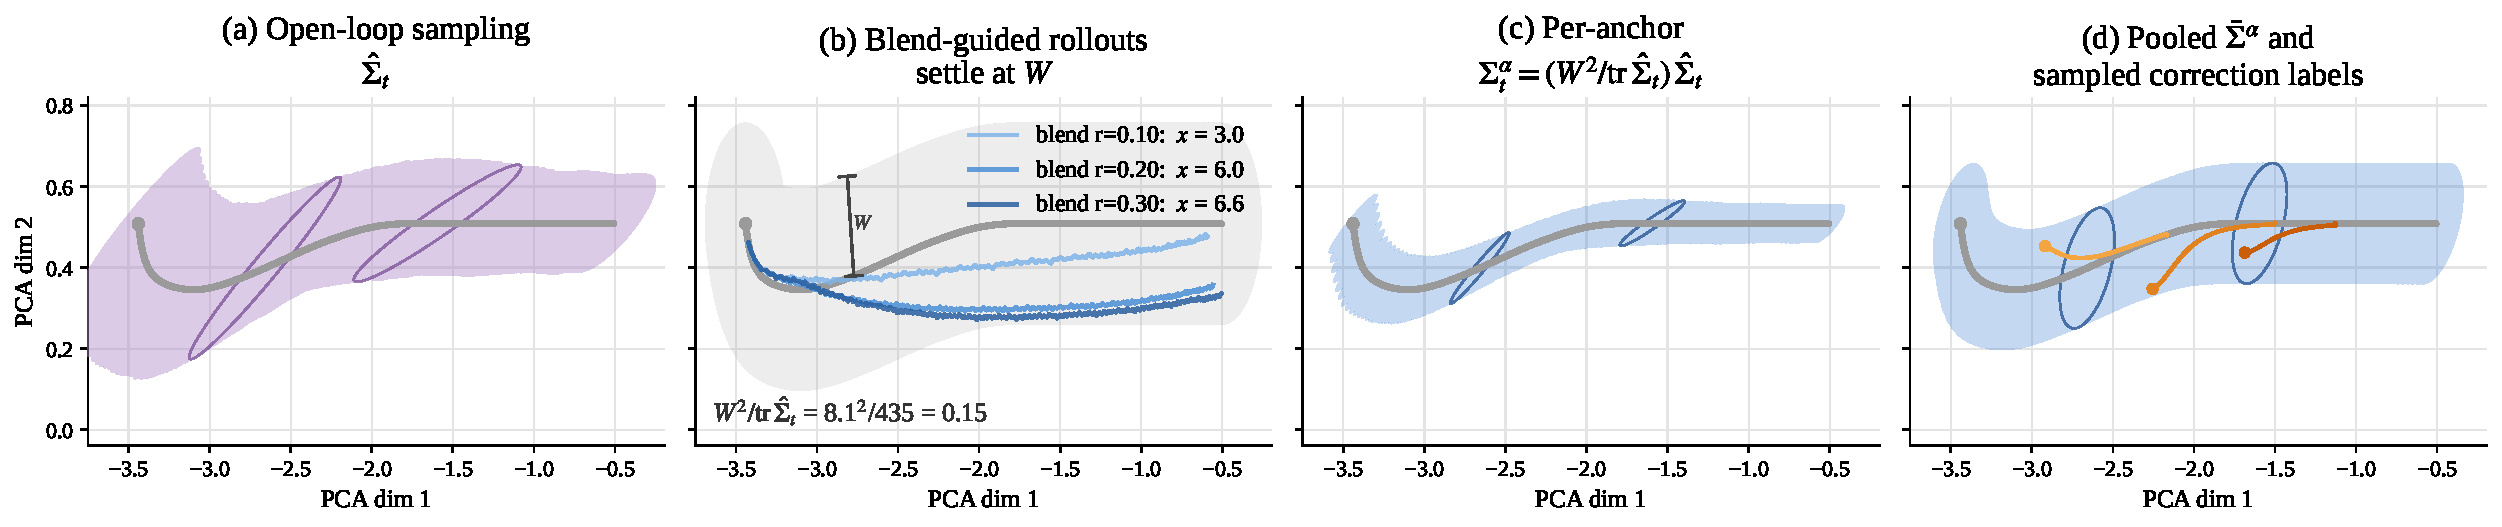
\includegraphics[width=16.6cm]{calibration_panels.pdf}};
\begin{scope}[on background layer]
  \node[region, draw=cCal!60, fill=cCal!6, fit=(panels), inner sep=6pt] (calbox) {};
\end{scope}
\node[lab, text=cCal!70!black, anchor=south west] at ($(calbox.north west)+(0.15,0.02)$) {\textbf{Policy calibration + augmentation} \quad offline, in simulation, no expert required};
% pi_theta chips over the panels that query the policy (a) and (b)
\node[chip] at ($(panels.north west)+(0.95,-1.05)$) {$\pi_\theta$};
\node[chip] at ($(panels.north west)+(0.25*16.6cm+0.95cm,-1.05)$) {$\pi_\theta$};
\node[data, fill=cCal!22, right=0.5cm of calbox.east] (Dhat) {Calibrated\\recovery $\hat{\mathcal{D}}_k$};
\draw[flow] (calbox.east) -- (Dhat);

% ================= Connections between rows =================
\draw[loop] (Dk.south) -- (Dk.south |- calbox.north);
\coordinate (p1) at ($(train.south)+(0,-0.8)$); \coordinate (p2) at ($(calbox.west)+(-0.5,0)$);
\draw[loop] (train.south) -- (p1) -- (p2 |- p1) -- (p2) -- (calbox.west);
\node[chip] at (p2 |- {$(p1)!0.5!(p2)$}) {$\pi_\theta$};
\coordinate (bot) at ($(calbox.south)+(0,-0.55)$);
\coordinate (agx) at ($(Dhat.east)+(0.45,0)$);
\coordinate (lx) at (1.15,0); \coordinate (tin) at ($(train.west)+(0,-0.45)$);
\draw[loop] (Dk.east) -- (agx |- Dk.east) -- (agx |- bot) -- node[lab, below, text=black!70, pos=0.5] {\textbf{Aggregate} $\;\mathcal{D}_0 \cup \mathcal{D}_{1..k} \cup \hat{\mathcal{D}}_{1..k}$} (lx |- bot) -- (lx |- tin) -- (tin);
\draw[line width=1.4pt, draw=black!60, rounded corners=8pt] (Dhat.south) -- (Dhat.south |- bot);
\fill[black!60] (Dhat.south |- bot) circle (2pt);
\node[lab, text=black!60, anchor=west] at ($(agx |- Dk.east)+(0.1,-0.55)$) {$\mathcal{D}_k$};
\end{tikzpicture}
\end{document}
